\section{Konzept}
Hier wird ein Konzept mit Mock Ups und Architektur entstehen

\subsection{Auswahl von Erfassungsmöglichkeiten}
\subsectionauthor{Lukas Seemann}
Nachdem im letzten Kapitel bereits verschiedene Möglichkeiten vorgestellt wurden, mit denen Emotionsindizien von Menschen erfasst werden können, wird eine Auswahl auf die für die Arbeit relevanten Möglichkeiten getroffen. Dies erfolgt mithilfe einer Nutzwertanalyse. \newline
Hierbei werden alle Alternativen aufgelistet. Anschließend werden verschiedene Kategorien definiert, anhand denen die einzelnen Alternativen bewertet werden. Die Kategorien werden anschließend mit einer Gewichtung versehen, wobei insgesamt 100\% erreicht werden. In jeder Kategorie müssen für jede Möglichkeit Punkte auf einer Skala von eins bis fünf vergeben werden. Nachdem auf diese Art und Weise alle Alternativen bewertet wurden, wird die Nutzwertanalyse ausgewertet. Hierzu wird die Bewertung in einer Kategorie mit der zugehörigen Gewichtung multipliziert, wodurch man die gewichtete Bewertung erhält. Die Addidtion der gewichteten Bewertungen einer Möglichkeit ergibt die Gesamtbewertung. Anhand dieser Gesamtbewertungen kann festgestellt werden, welche der aufgelisteten Kandidaten den höchsten Nutzwert besitzt. \newline
Die durchgeführte Nutzwertanaylse ist in Tabelle 1 abgebildet.
\begin{table}[h]
	\centering
	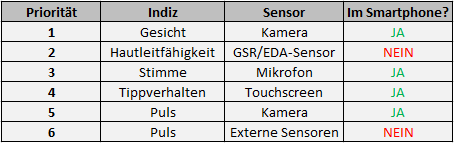
\includegraphics[width=14cm]{Bilder/prio.png}
	\caption[Nutzwertanalyse]{Nutzwertanalyse}
\end{table}%
\subsection{Priorisierung der Erfassungsmöglichkeiten}
\subsectionauthor{Lukas Seemann}
Im Anschluss an die Auswahl der Erfassungsmöglichkeiten werden diese Möglichkeiten nun priorisiert. In der folgenden Tabelle (Tabelle 1) ist die Priosierung abgebildet. \newline
\begin{table}[h]
	\centering
	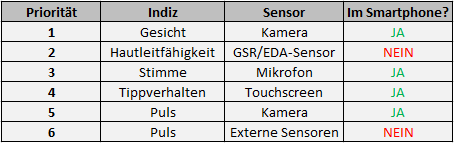
\includegraphics[width=14cm]{Bilder/prio.png}
	\caption[Priorisierung der Erfassungsmöglichkeiten]{Priorisierung der Erfassungsmöglichkeiten}
\end{table}%
\newline In der ersten Spalte ist die Priorität dargestellt. Je niedriger die Zahl ist, desto höher ist die Erfassungsmöglichkeit priorisiert. Die Möglichkeiten werden in der Reihenfolge der hier dargestellten Priorisierung thematisiert und letzten Endes in den Prototyp der mobilen Applikation integriert, um Daten zu erfassen. Je nachdem wie viel Zeit die einzelnen Features benötigen, können mehr und mehr Möglichkeiten der Datenerfassung in die App eingebaut werden, wenn sie noch im Zeitrahmen der Studienarbeit umsetzbar sind. Bei den einzelnen Möglichkeiten werden das Indiz, anhand dessen Rückschlüsse auf eine Emotion gemacht werden kann, und ein Sensor, der Daten zum Indiz für die App erfassen soll, aufgelistet. In der letzen Spalte ist festgehalten, ob der benötigte Sensor in den meisten aktuellen Smartphones bereits enthalten ist oder nicht. \newline
Die höchste Priorität hat das Indiz der Hautleitfähigkeit, die mithilfe von GSR- beziehungsweise EDA-Sensoren erfasst werden kann. Diese Art von Sensoren befinden sich nicht in handelsüblichen Smartphones, weshalb man hierzu externe Sensoren mit dem Handy verbinden muss. \newline
...

\subsection{Übertragung biometrischer Daten in Emotionscores}
\subsection{Auswertung der Scores zur Emotionsbestimmung}
\subsubsection{Kausalitätsregeln}
\subsubsection{Entscheidungsalgorithmus}
\subsectionauthor{Torben Brenner}
Ziel der Anwendung ist es, basierend auf zuvor aufgenommenen Daten eine Entscheidung zu fällen, welche Emotion der Nutzer der 
Anwendung aktuell empfinden könnte. Die Entscheidung muss dabei die verschiedenen Ergebnisse der Auswertungsebene einbeziehen
und aus diesen auf eine Emotion schließen. Deshalb muss eine Einheitliche Datenstruktur entwickelt werden, über die die Auswertungsebene
die Daten zur Verfügung stellt. \\
Die Entscheidung könnte hierbei über ein \textit{Scoring} entstehen. Dieses \textit{Scoring} müsste dabei auf der Auswertungsebene stattfinden, 
wobei jeder der Auswertungsalgorithmen ein \textit{Scoring} für die verschiedenen Emotionen angeben muss. Am Ende könnten z. Bsp. die verschiedenen 
\textit{Scorings} addiert und die Emotion mit dem höchsten \textit{Scoring} ausgewählt werden.
\subsection{Ionic Framework}
\subsubsection{Aufbau und Einsatz des Frameworks}
\subsubsectionauthor{Lukas Seemann}
Ionic ist ein unter der MIT License stehendes Open-Source-Framework, das zur Entwicklung von plattformübergreifenden, mobilen Applikationen dient. Mit Ionic entwickelte Apps sind damit unter anderem auf Endgeräten lauffähig, die die Betriebssysteme Android, iOS und Windows Phone benutzen. \footcite{Ion18a}
\begin{figure}[h]
	\centering
	
\includegraphics[width=11cm]{Bilder/ionic.png}
	\caption[Ionic Framework - Logo]{Ionic Framework - Logo\footnotemark}
\end{figure}%
\footcitetext{Wik18}
\newline
Aktuell befindet sich das Framework in der Version 3.9.2\footcite[Vgl. ][]{Ion18b} und befindet sich in stetiger Weiterentwicklung. Das Ionic Framework basiert wiederum auf Angular, einem Framework für die Entwicklung von Web-Applikationen. Dementsprechend nutzen Ionic-Anwendungen in der Web-Entwicklung etablierte Technologien wie HTML 5, CSS und JavaScript. \footcite[Vgl. ][]{Ion18c} Wie auch im Angular Framework, wird auch die Programmiersprache TypeScript verwendet, die auf JavaScript aufbaut, sich in der Syntax sehr stark mit JavaScript ähnelt und zusätzliche Optionen zur Typisierung von Variablen oder Funktionen anbietet. \footcite[Vgl. ][]{Til17} \newline
Ionic-Anwendungen sind im Wesentlichen normale Webanwendungen, die von jedem JavaScript-fähigen Browser ausgeführt werden können. Während mithilfe von Ionic das Frontend der Anwendung festgelegt wird, kann anschließend mit Apache Cordova die Plattformunabhängigkeit umgesetzt werden. Apache Cordova bewirkt, dass sich die Webanwendungen wie native Android-, iOS- oder Windows Phone-Applikationen anfühlen. Egal auf welcher Plattform die Ionic-Anwendung installiert wird, es wird die selbe Code-Basis verwendet. Diese wird dann vor dem Installieren von Cordova so angepasst, dass sie auf den Endgeräten ausgeführt werden können. \footcite{Ion18d}
\subsubsection{Gründe für die Verwendung}

\subsection{Architektur der mobilen Applikation}
